% !TeX spellcheck = en_US

\documentclass{../UTNetLab}

\title{Linux and TCP/IP Networking}
\labnumber{1}
\newcommand\reference{
   S. Panwar, S. Mao, J.-dong Ryoo, and Y. Li, “Linux and TCP/IP networking,” in TCP/IP Essentials: A Lab-Based Approach, Cambridge: Cambridge University Press, 2004, pp. 26–42.
}

\begin{document}
\section*{Objectives}
\begin{itemize}
    \item Getting acquainted with the lab environment.
    \item Getting acquainted with the Linux operating system.
    \item Preview of some TCP/IP diagnostic tools.
    \item Capturing and analyzing the link layer, IP, and TCP headers.
    \item Understanding the concept of encapsulation.
    \item Understanding the concept of multiplexing using \textit{port numbers}, the IP \textit{protocol} field, and the Ethernet \textit{frame type} field.
    \item Understanding the client–server architecture.
\end{itemize}

\section*{Systems Configuration}
Launch GNS3 and make a network as below.
You can use \lstbash[emph={eth0},morekeywords={[3]netmask}]{ifconfig eth0 192.168.0.1 netmask 255.255.255.0} to set ip.
\begin{center}
    \begin{minipage}{0.48\textwidth}
        \begin{flushleft}
            \begin{table}[H]
                \caption{The IP addresses of the hosts (Table~1.2)}
                \centering
                \begin{tabular}{ c c c }
                    \hline \hline
                    Host & IP Address     & Subnet Mask   \\
                    \hline
                    h0   & 128.238.66.100 & 255.255.255.0 \\
                    h1   & 128.238.66.101 & 255.255.255.0 \\
                    h2   & 128.238.66.102 & 255.255.255.0 \\
                    h3   & 128.238.66.103 & 255.255.255.0 \\
                    h4   & 128.238.66.104 & 255.255.255.0 \\
                    h5   & 128.238.66.105 & 255.255.255.0 \\
                    h6   & 128.238.66.106 & 255.255.255.0 \\
                    h7   & 128.238.66.107 & 255.255.255.0 \\
                    \hline \hline
                \end{tabular}
            \end{table}
        \end{flushleft}
    \end{minipage}
    \begin{minipage}{0.48\textwidth}
        \begin{flushright}
            \begin{figure}[H]
                \centering
                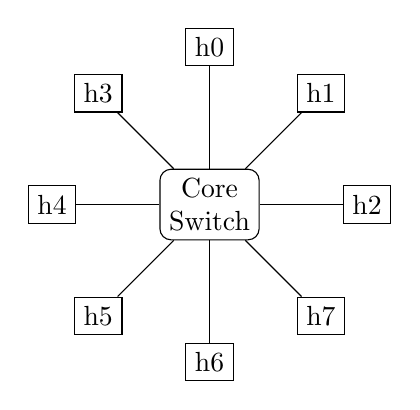
\begin{tikzpicture}
                    \node[draw,align=center,rounded corners] (s) at (0,0){Core\\Switch};
                    \node[draw] (h0) at (0,2){h0};
                    \node[draw] (h1) at ({sqrt(2)},{sqrt(2)}){h1};
                    \node[draw] (h2) at (2,0){h2};
                    \node[draw] (h3) at (-{sqrt(2)},{sqrt(2)}){h3};
                    \node[draw] (h4) at (-2,0){h4};
                    \node[draw] (h5) at (-{sqrt(2)},-{sqrt(2)}){h5};
                    \node[draw] (h6) at (0,-2){h6};
                    \node[draw] (h7) at ({sqrt(2)},-{sqrt(2)}){h7};

                    \draw (h0) -- (s);
                    \draw (h1) -- (s);
                    \draw (h2) -- (s);
                    \draw (h3) -- (s);
                    \draw (h4) -- (s);
                    \draw (h5) -- (s);
                    \draw (h6) -- (s);
                    \draw (h7) -- (s);
                \end{tikzpicture}
                \caption{A single segment network (Figure~1.3)}
            \end{figure}
        \end{flushright}
    \end{minipage}
\end{center}

\section{Telnet Service}
Run \lstbash{ps -e} to list the processes running in the \textit{h1}.
After starting a new process by running \lstbash{telnet} in another command window (open new auxiliary console), execute \lstbash{ps -e} again in a third window to see if there is any change in its output.

Find the process id of the \lstbash{telnet} process you started, by:
\begin{lstlisting}
ps -e | grep telnet
    \end{lstlisting}
Then use \lstbash[emph={process-id-of-telnet}]{kill process-id-of-telnet} to terminate the \lstbash{telnet} process.

\begin{report}
    \item What is Internet Service Daemon (\lstbash{inetd})?

    \item Is \lstbash{inetd} started in your system? Why?

    \item Is \lstbash{xinetd} started in your system? What is its PID?
\end{report}

\section{Default Network Services}
Display the file \path{/etc/services} on the \textit{h1} screen, using:
\begin{lstlisting}
more /etc/services
    \end{lstlisting}
Then in another console (Auxiliary console), use the redirect operator to redirect the \lstbash{more} output to
a file using \lstbash{more /etc/services > ser-more}.
Compare the file \path{ser-more} with the original \lstbash{more} output in the other command window.

Copy \path{/etc/services} file to a local file named \path{ser-cp} in your working directory (use \lstbash{pwd} to see working directory path),
using \lstbash{cp /etc/services ser-cp}.
Compare files \path{ser-more} and \path{ser-cp}, using \lstbash{cmp ser-more ser-cp}.
Are these two files identical?

Concatenate these two files using \lstbash{cat ser-more ser-cp > ser-cat}.

Display the file sizes using \lstbash{ls -l ser*}.
Save the output.

\begin{report}
    \item What are the sizes of files \path{ser-more}, \path{ser-cp}, and \path{ser-cat}?
\end{report}

\section{Network Command Manual}
Read the \lstbash{man} pages for the following programs:
\begin{multicols}{3}
    \begin{enumerate}
        \item \lstbash{arp}
        \item \lstbash{arping}
        \item \lstbash{ifconfig}
        \item \lstbash{tcpdump}
        \item \lstbash{ping}
        \item \lstbash{netstat}
        \item \lstbash{route}
        \item \lstbash{wireshark}
        \item \lstbash{iptables}
    \end{enumerate}
\end{multicols}
Study the different options associated with each command.
Throughout this lab you will use these commands rather extensively.

\begin{report}
    \item Explain the above commands briefly.
    (Two or three sentences per command would be adequate.)
\end{report}

\section{Packet Capturing}
% fixme: content
In this exercise, we will use \lstbash{tcpdump} to capture a packet containing the link, IP, and TCP headers and use \lstbash{wireshark} to analyze this packet.

First, run \lstbash{tcpdump -enx -w dump.pcap} in the \textit{h1}.
You will not see any \lstbash{tcpdump} output, since the \lstbash{-w} option is used to write the output to the \path{dump.pcap} file.

Then, you may want to run \lstbash{telnet 128.238.66.102} in the \textit{h1} to generate some TCP traffic.\footnote{Remember to run \lstbash{/etc/init.d/xinetd restart} in the \textit{h2} to start telnet server on it.}
After you login to \textit{h2} (use \textbf{netlab} for username and password), terminate the \lstbash{telnet} session and terminate the \lstbash{tcpdump} program.
Next, you will use \lstbash{tcpdump} or \lstbash{wireshark} to open the packet trace captured by \lstbash{tcpdump} and analyze the captured packets.
To do this, use this command \lstbash{tcpdump -r dump.pcap} to see content of \path{dump.pcap} or see with GUI \lstbash{wireshark dump.pcap &}\footnote{To use \lstbash{wireshark} in isolated \lstbash{docker} space, you need to copy file from  \lstbash{docker} space to your PC}.
The \lstbash{wireshark} Graphical User Interface (GUI) will pop up and the packets captured by \lstbash{tcpdump} will be displayed.
Select any one of the packets that contain the link, IP, and TCP headers.
In GNS3 you can capture ans see packet with right click on wire and select \textit{Start Capture}.

\begin{report}
    \item What is the value of the \texttt{protocol} field in the IP header of the packet you saved?
    What is the use of the \texttt{protocol} field?

    \item What is the value of the \texttt{frame type} field in an Ethernet frame carrying an IP datagram?
\end{report}

\section{\texttt{ARPing}}
This time we will run \lstbash{wireshark} to capture an ARP request and an ARP reply in real-time.
Simply run \lstbash{wireshark} on the \textit{h1} link with right click and select \textbf{start capture} item to start capturing\footnote{On physical machine, can start capture with \lstbash{wireshark &} command.}.
If there is no arp requests and replies in the network, generate some using \lstbash{arping 128.238.66.102} command in the \textit{h1} terminal.

Now you should see several ARP replies in the \lstbash{arping} output.

\begin{report}
    \item What is the value of the \texttt{frame type} field in an Ethernet frame carrying an ARP request and in an Ethernet frame carrying an ARP reply, respectively?

    \item What is the use of the \texttt{frame type} field?
\end{report}

\section{Packet Filtering}
Using the \lstbash{tcpdump} utility, capture any packet on the LAN and see the output format
for different command-line options.
Study the various expressions for selecting
which packets to be dumped.

For this experiment, use the \lstbash{man} page for \lstbash{tcpdump} to find out the options and
expressions that can be used.

If there is no traffic on the network, you may generate traffic with some applications
(e.g.\ \lstbash{telnet}, \lstbash{ping}, etc.).

\begin{report}
    \item Explain briefly the purposes of the following \lstbash{tcpdump} expressions.
\end{report}

% todo: make sample traffic
If you are using \lstbash{tcpdump}, explain the following filters:
\begin{itemize}
    \item \lstbash{tcpdump udp port 520}
    \item \lstbash{tcpdump -x -s 120 ip proto 89}
    \item \lstbash[emph={ip-addr1, ip-addr2, ip-addr3}]{tcpdump -x -s 70 host ip-addr1 and (ip-addr2 or ip-addr3)}
    \item \lstbash[emph={ip-addr1, ip-addr2}]{tcpdump -x -s 70 host ip-addr1 and not ip-addr2}
\end{itemize}

If you are using \lstbash{wireshark} explain the following filters:
\begin{itemize}
    \item \lstgeneric{udp.port == 520}
    \item \lstgeneric{ip.proto == 89}
    \item \lstgeneric[emph={ip-addr1, ip-addr2, ip-addr3}]{ip.addr == ip-addr1 and (ip.addr == ip-addr2 or ip.addr == ip-addr3)}
    \item \lstgeneric[emph={ip-addr1, ip-addr2}]{ip.addr == ip-addr1 and not ip.addr ip-addr2}
\end{itemize}

\section{Connection Port}
Run \lstbash{wireshark} on the \textit{h1} link and select an interface to capture packets between hosts.

Execute a TCP utility, \lstbash{telnet} for example, in another command window:
\begin{lstlisting}
telnet 128.238.66.102
    \end{lstlisting}

\begin{report}
    \item What are the port numbers used by the \textit{h1} (local machine) and the \textit{h2} (remote machine)?

    \item Which port numbers matches the port number listed for \lstbash{telnet} in the \path{/etc/services} file?
\end{report}

\section{Random Port}
Run \lstbash{wireshark} on the \textit{h1} link and select an interface to capture packets between hosts.

Then, \lstbash{telnet} to the \textit{h2} from a second command window (Auxiliary console) by typing \lstbash{telnet 128.238.66.102}.
Again issue the same \lstbash{telnet 128.238.66.102} command from a third command window.
Now you are opening two \lstbash{telnet} sessions to \textit{h2} simultaneously, from two different command windows.
% On each telnet terminal, run \lstbash{pwd} to generate traffic.

Check the port numbers being used on both sides of the two connections from the output in the \lstbash{wireshark} window.

\begin{report}
    \item When you have two \lstbash{telnet} sessions with your machine, what port number is used on the \textit{h2} (remote machine)?

    \item Are both sessions connected to the same port number on the \textit{h2} (remote machine)?

    \item What port numbers are used in the \textit{h1} (local machine) for the first and second \lstbash{telnet}, respectively?

    \item Explain briefly what a \lstbash{socket} is.
\end{report}
\end{document}